\documentclass[sigconf]{acmart}
% =============================================================================
% Template setup — participants normally do not edit this file.
% Author content belongs in main.tex; citations belong in main.bib.
% \documentclass lives in main.tex so Overleaf does not treat this file as root.
% =============================================================================

% --- Competition / non-ACM-submission friendly rights metadata -------------
\setcopyright{none}
\settopmatter{printacmref=false}
\acmConference[Kaggle Competition]{Filament Segmentation Challenge}{2026}{\href{https://www.kaggle.com/competitions/filament-segmentation-2026}{kaggle.com/competitions/filament-segmentation-2026}}
\acmBooktitle{Competition Report}
\acmDOI{}
\acmISBN{}

% --- Author guidance text --------------------------------------------------
% \guide{...} is gray italic while \guideStyletrue; omitted from the PDF if false.
% Flip the switch in main.tex after % =============================================================================
% Template setup — participants normally do not edit this file.
% Author content belongs in main.tex; citations belong in main.bib.
% \documentclass lives in main.tex so Overleaf does not treat this file as root.
% =============================================================================

% --- Competition / non-ACM-submission friendly rights metadata -------------
\setcopyright{none}
\settopmatter{printacmref=false}
\acmConference[Kaggle Competition]{Filament Segmentation Challenge}{2026}{\href{https://www.kaggle.com/competitions/filament-segmentation-2026}{kaggle.com/competitions/filament-segmentation-2026}}
\acmBooktitle{Competition Report}
\acmDOI{}
\acmISBN{}

% --- Author guidance text --------------------------------------------------
% \guide{...} is gray italic while \guideStyletrue; omitted from the PDF if false.
% Flip the switch in main.tex after % =============================================================================
% Template setup — participants normally do not edit this file.
% Author content belongs in main.tex; citations belong in main.bib.
% \documentclass lives in main.tex so Overleaf does not treat this file as root.
% =============================================================================

% --- Competition / non-ACM-submission friendly rights metadata -------------
\setcopyright{none}
\settopmatter{printacmref=false}
\acmConference[Kaggle Competition]{Filament Segmentation Challenge}{2026}{\href{https://www.kaggle.com/competitions/filament-segmentation-2026}{kaggle.com/competitions/filament-segmentation-2026}}
\acmBooktitle{Competition Report}
\acmDOI{}
\acmISBN{}

% --- Author guidance text --------------------------------------------------
% \guide{...} is gray italic while \guideStyletrue; omitted from the PDF if false.
% Flip the switch in main.tex after \input{preamble}.
%
% Do not use \guide{...} for \email{...}.
\usepackage{xcolor}
\newif\ifguideStyle
\guideStyletrue
\newcommand{\guide}[1]{%
  \ifguideStyle
    {\color{gray!65}\itshape #1}%
  \fi
}

% --- Math ------------------------------------------------------------------
% Do NOT load amssymb (or amsfonts): acmart already loads newtxmath, which
% defines the same symbols (e.g. \Bbbk) and causes a conflict on Overleaf.
% amsmath is already provided by acmart; mathtools extends it.
\usepackage{mathtools}

% --- Figures ---------------------------------------------------------------
% graphicx is already loaded by acmart
\usepackage{subcaption}

% --- Tables ----------------------------------------------------------------
% booktabs is already loaded by acmart
\usepackage{tabularx}
\usepackage{multirow}

% --- Bibliography style is set in main.tex (ACM-Reference-Format) ----------
.
%
% Do not use \guide{...} for \email{...}.
\usepackage{xcolor}
\newif\ifguideStyle
\guideStyletrue
\newcommand{\guide}[1]{%
  \ifguideStyle
    {\color{gray!65}\itshape #1}%
  \fi
}

% --- Math ------------------------------------------------------------------
% Do NOT load amssymb (or amsfonts): acmart already loads newtxmath, which
% defines the same symbols (e.g. \Bbbk) and causes a conflict on Overleaf.
% amsmath is already provided by acmart; mathtools extends it.
\usepackage{mathtools}

% --- Figures ---------------------------------------------------------------
% graphicx is already loaded by acmart
\usepackage{subcaption}

% --- Tables ----------------------------------------------------------------
% booktabs is already loaded by acmart
\usepackage{tabularx}
\usepackage{multirow}

% --- Bibliography style is set in main.tex (ACM-Reference-Format) ----------
.
%
% Do not use \guide{...} for \email{...}.
\usepackage{xcolor}
\newif\ifguideStyle
\guideStyletrue
\newcommand{\guide}[1]{%
  \ifguideStyle
    {\color{gray!65}\itshape #1}%
  \fi
}

% --- Math ------------------------------------------------------------------
% Do NOT load amssymb (or amsfonts): acmart already loads newtxmath, which
% defines the same symbols (e.g. \Bbbk) and causes a conflict on Overleaf.
% amsmath is already provided by acmart; mathtools extends it.
\usepackage{mathtools}

% --- Figures ---------------------------------------------------------------
% graphicx is already loaded by acmart
\usepackage{subcaption}

% --- Tables ----------------------------------------------------------------
% booktabs is already loaded by acmart
\usepackage{tabularx}
\usepackage{multirow}

% --- Bibliography style is set in main.tex (ACM-Reference-Format) ----------

\guideStylefalse
\begin{document}
\title[Quality-Aware Solar Filament Segmentation]{Quality-Aware Multiscale Instance Segmentation and Selective Mask Refinement for Solar Filament Delineation}
\subtitle{A Solution to the Solar Filament Segmentation Challenge 2026}
\author{Lighittha Pappusamy Rathika}
\affiliation{\institution{Vellore Institute of Technology, Chennai}\city{Chennai}\country{India}}
\email{ligpersonalmail@gmail.com}
\author{Prithivraj Selvakumar}
\affiliation{\institution{Vellore Institute of Technology, Chennai}\city{Chennai}\country{India}}
\email{theprithivrajs@gmail.com}
\renewcommand{\shortauthors}{Rathika and Selvakumar}
\begin{abstract}
This report describes a quality-aware instance-segmentation system for the Solar Filament Segmentation Challenge 2026. Two solar-adapted YOLO11m segmentation detectors operate on a resized full-disk GONG H$\alpha$ image and overlapping native-resolution windows; nonmaximum suppression, overlap arbitration, a learned 69-feature quality ensemble, and selective prompt-conditioned mask refinement produce nonoverlapping filament instances. The archived 1,093-instance submission achieved a user-confirmed public leaderboard Panoptic Quality (PQ) of \textbf{0.39} (rounded display). For a reproducible analysis on 51 historically reused, acquisition-day-separated audit scenes, the reconstructed pipeline attains \textbf{PQ 0.4589}; removing the quality ranker or selective mask refiner lowers PQ to 0.4490 and 0.4469, respectively. Across three refits, detector-support and image-appearance features are more consequential than the tested neighborhood features. We provide fixed-checkpoint ablations, paired-day descriptive bootstrap intervals, expert-disagreement analysis, instance-size recall, case visualizations, and a reproducibility manifest. These local results are distinct from the public score and do not constitute untouched-test evidence.
\end{abstract}
\maketitle
\section{Introduction}
The Solar Filament Segmentation Challenge 2026 \cite{filament-segmentation-2026} evaluates the delineation of individual filaments in full-disk 2048$\times$2048 GONG H$\alpha$ observations using the MAGFiLO annotations \cite{ahmadzadeh2024dataset}. Filaments are narrow, often fragmented structures whose apparent segmentation accuracy depends both on mask geometry and on assigning pixels to the correct instance. Pixel-level foreground coverage alone can therefore conceal missed instances, duplicates, or false positives. We target Panoptic Quality (PQ) \cite{kirillov2019}, emphasizing the trade-off between overlap quality and reliable instance recognition.

The submitted solution combines (i) global and native-window segmentation, (ii) quality-aware acceptance of candidate instances, and (iii) selective correction of accepted mask boundaries. Rather than treating every investigated network as a contribution, we report controlled removal and replacement experiments against the frozen 0.39-public-score V25 pipeline. Our evidence also documents when a seemingly useful curve-proposal mechanism \emph{does not} increase PQ.

\section{Development Trajectory and Failed Hypotheses}\label{sec:history}
The historical work began with semantic models and compact instance detectors at approximately 0.31--0.32 public PQ. Native-window inference subsequently established a 0.34 control (V7), while the V8 tile-specialist experiment encountered a JSON tuple/list cache error that invalidated its immediate evaluation. A separate ridge-pixel learner (V9) yielded a 0.31 public output and a V10 baseline reconstruction gave 0.33. The V12--V15 candidate-action studies exposed an important pitfall: an apparent local gain against a reconstructed baseline was not proof of improvement over the exact scored CSV. A clean-slate V16 study reached local PQ 0.3899 with YOLO11m but only about 0.33 publicly, demonstrating local/leaderboard disagreement.

Later global/native multiscale training produced the reported V22 0.37 public recipe, followed by V24 0.38 with learned quality control and the final V25 0.39. In a historical audit, V28 high-resolution detector fusion improved V25 by at most +0.0003 local PQ and a V29 novelty-credit ranker by +0.0008; neither was promoted. These findings motivated final emphasis on avoiding false positives and refining only accepted masks, rather than assuming more proposals imply better PQ. Development milestones are descriptive, not matched-dataset experiments; the appendix-length chronology and failure evidence are in the extended companion manuscript.
\begin{figure}[t]
\centering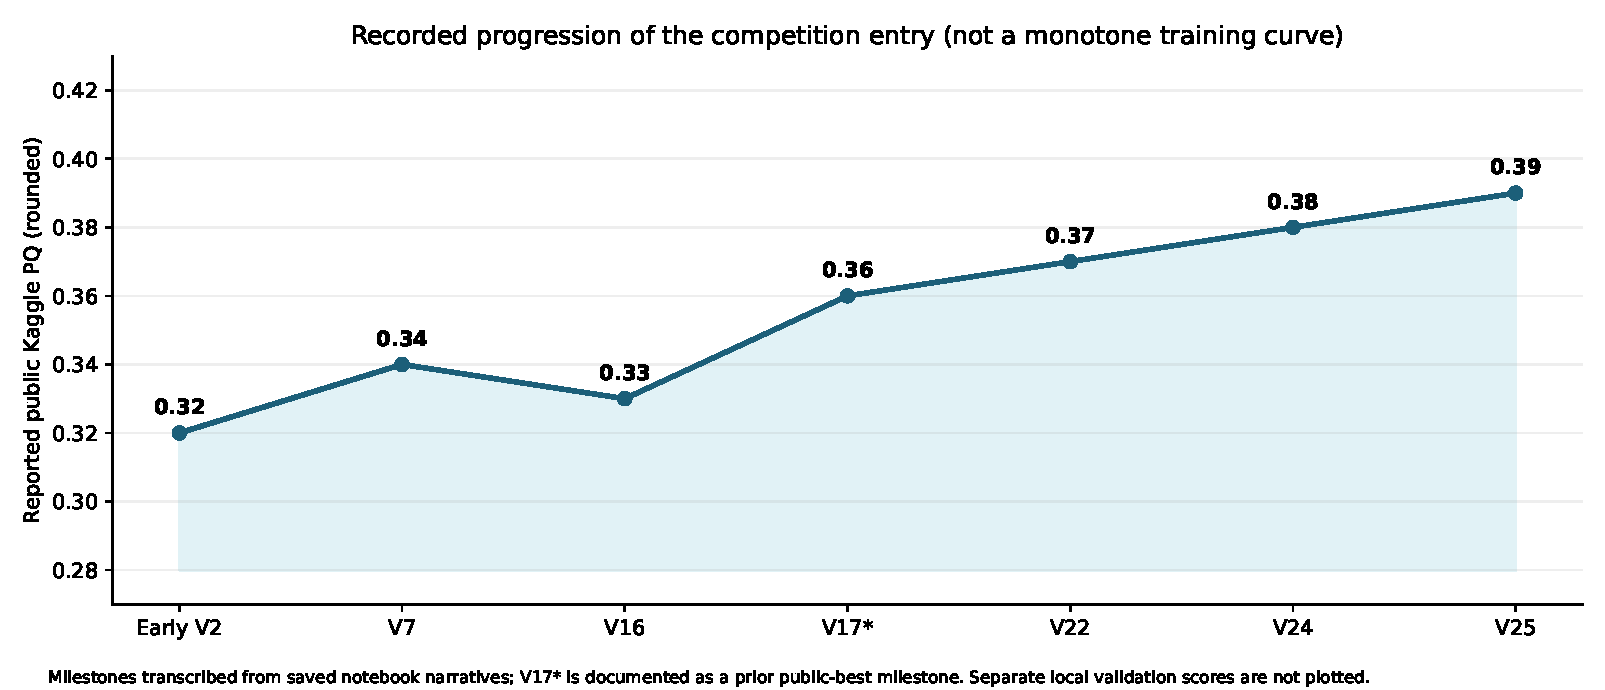
\includegraphics[width=\columnwidth]{development.pdf}
\caption{Notebook-recorded public milestones, distinct from the local audit and not a monotonic training trace.}\label{fig:history}
\end{figure}
\section{Methodology}\label{sec:methodology}
\subsection{Data, provenance, and split discipline}
The competition provides 707 labeled training scenes, 180 hidden-label test scenes, and multiple expert annotation versions for some images. The two YOLO11m-seg checkpoints originated from the historical V20 training split, leaving 104 scenes grouped by acquisition day outside their training images. Later method development used these 104 scenes repeatedly. The final study divides them into 53 calibration and 51 audit scenes (46 audit acquisition days). This last partition separates the ranker-refit fitting procedure from its evaluation but \emph{cannot} be regarded as an untouched independent holdout. No test-set annotations are read by the code.

\subsection{Multiscale detector proposals}
The two fixed YOLO11m-seg networks (22.36M parameters each) operate on the same H$\alpha$ image using complementary receptive fields. The global checkpoint processes full-disk images at a network resolution of 1792 pixels. The native checkpoint processes four overlapping 1280$\times$1280 windows, each resized to 1024 pixels for inference. Both use raw confidence 0.08, raw NMS IoU 0.72, class-agnostic NMS, retina masks, and at most 120 detections per inference view. Every predicted mask is remapped to the original 2048$\times$2048 coordinates and encoded in COCO compressed run-length encoding (RLE).

The frozen detector decoder filters full-image detections at confidence 0.24 and tiled detections at 0.42, removes candidates smaller than 200 pixels, rejects interior-window truncations, sorts with a 0.08 native-tile score bonus, and suppresses duplicate masks at IoU 0.50. Sequential occupancy arbitration retains only the unclaimed mask area, subject to a minimum free fraction of 0.45. These values identify the historical configuration and were not retuned using the final audit table.

\begin{figure}[t]
\centering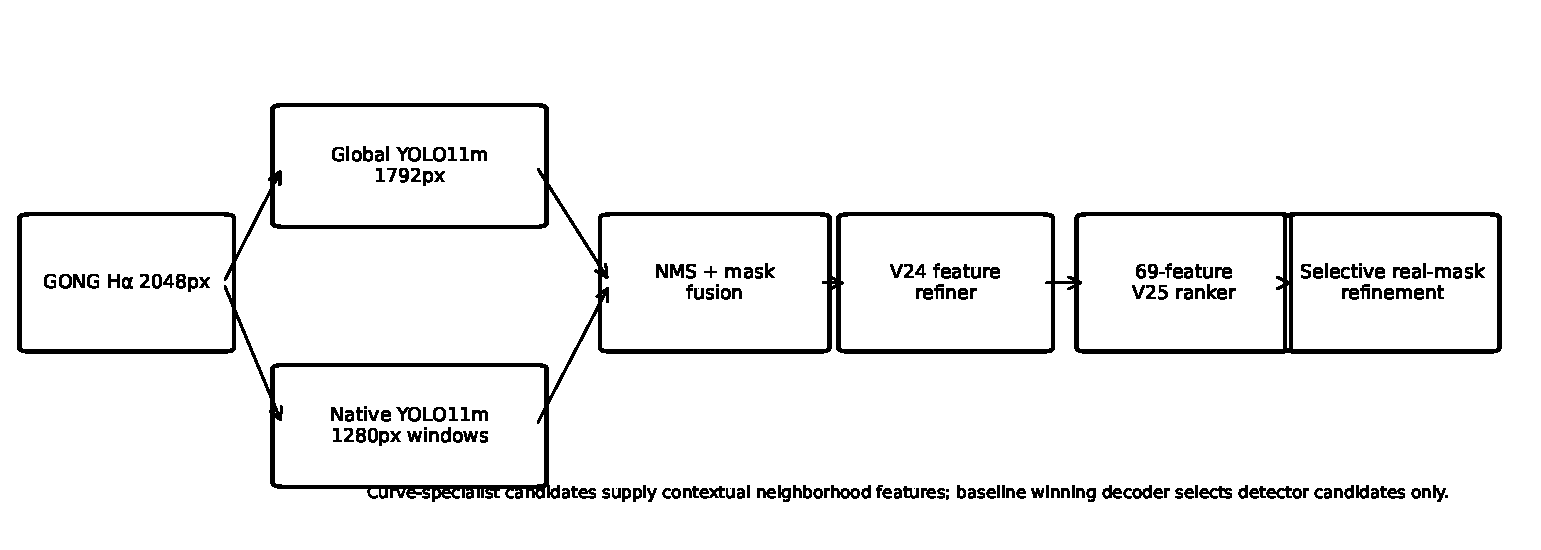
\includegraphics[width=\columnwidth]{pipeline.pdf}
\caption{Frozen multiscale V25 inference pipeline. The curve specialist supplies candidate/context information; its detections were \emph{not} directly included by the original winning output decoder.}\label{fig:pipeline}
\end{figure}

\subsection{Quality-aware selection and refinement}
A 4-channel prompt-conditioned residual-encoder U-Net provides local refinement-derived features. Candidate quality is estimated from \textbf{69 measurements}: detector confidence and agreement, shape and topology (including skeleton measures), H$\alpha$ appearance, spatial context and other geometric cues. The stored quality ensemble and its fixed threshold 0.38 retain a subset of the detector-generated candidates. Accepted candidates with predicted quality at least 0.50 are passed through a second prompt-conditioned mask refiner; geometric constraints reject implausible changes, and occupancy clipping ensures nonoverlapping final instances. The architecture contains a trained curve specialist for additional evidence, but the original final decoder accepted detector-origin instances only.

\subsection{Public-submission identity}
The actual user-confirmed public-score-0.39 artifact contains \textbf{1,093 filament-instance RLE rows} for the 180 hidden-label scenes, with SHA-256 prefix \texttt{ac470fbfa0e2ca5f2d}. The full SHA-256 and checkpoint hashes are preserved in the reproducibility archive. This scored file is not silently replaced with reconstructed masks. Exact test-output parity was \emph{not} exercised in the present ablation run.

\section{Evaluation}\label{sec:evaluation}
\subsection{Metrics and controlled ablations}
For each expert version, an instance match requires IoU$>0.5$ after one-to-one assignment. Define $\mathrm{PQ}=\sum_{(p,g)\in TP}\mathrm{IoU}(p,g)\,/\,[|TP|+\tfrac12|FP|+\tfrac12|FN|]$, with $\mathrm{SQ}$ the mean matched IoU and $\mathrm{RQ}$ the recognition fraction. Counts are pooled across expert versions using the historical local evaluator. Foreground Dice is computed separately. Official competition-evaluator parity has \emph{not} been established.

\begin{table}[t]
\caption{Same-scene historical audit (51 scenes). PQ values are local, \emph{not} public leaderboard scores. All stages use actual frozen learned weights.}\label{tab:ablations}
\centering\small
\begin{tabular}{lrr}
\toprule
Configuration & PQ & $\Delta$PQ \\
\midrule
Full reconstructed V25 & \textbf{0.4589} & --- \\
No curve context & 0.4584 & $-0.0005$ \\
Add curve detections & 0.4567 & $-0.0022$ \\
No quality ranker & 0.4490 & $-0.0099$ \\
No real-mask refiner & 0.4469 & $-0.0120$ \\
V24 quality gate & 0.4441 & $-0.0147$ \\
Two-detector fusion & 0.4369 & $-0.0220$ \\
Global detector alone & 0.4335 & $-0.0254$ \\
Native detector alone & 0.3631 & $-0.0957$ \\
\bottomrule
\end{tabular}
\end{table}

The final pipeline yields SQ 0.6799 and RQ 0.6749, corresponding to 409 matched instances, 164 false positives, and 230 false negatives when summed across expert versions. Removing the real-mask refiner decreases PQ by 0.0120 (95\% descriptive acquisition-day bootstrap difference interval $[-0.0183,-0.0066]$); removing the quality ranker decreases PQ by 0.0099 (interval $[-0.0202,-0.0002]$). Both intervals are conditional on historical model development and are \emph{not} confirmatory confidence statements about new solar data.

\begin{figure}[t]
\centering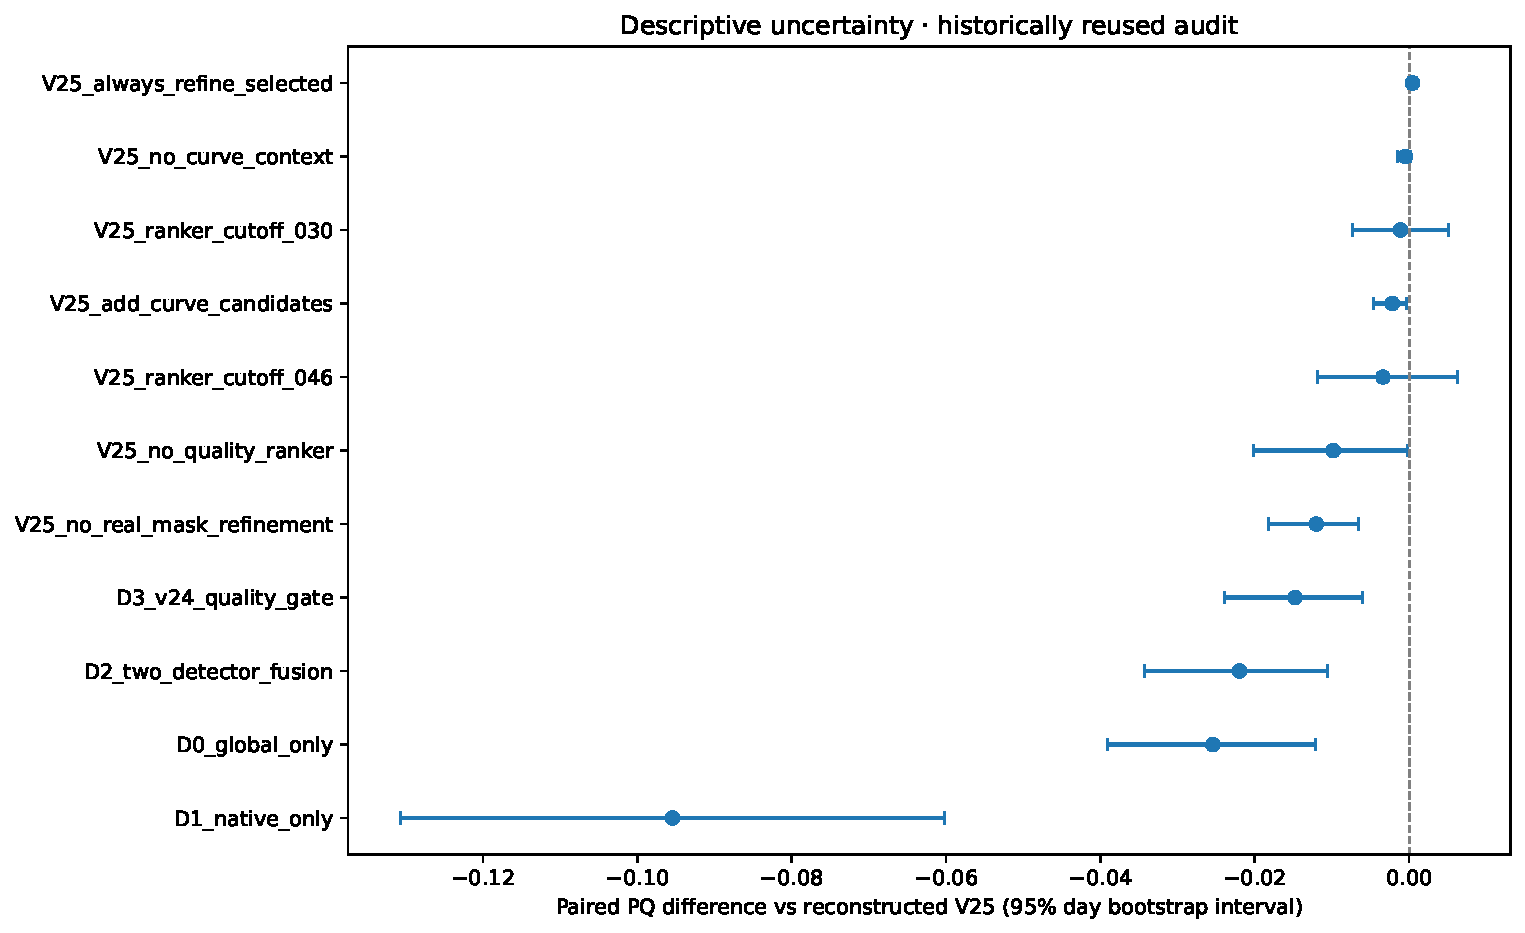
\includegraphics[width=.98\columnwidth]{bootstrap.pdf}
\caption{Day-cluster bootstrap differences against the reconstructed V25 pipeline, using the repeatedly consulted historical audit. Intervals quantify within-audit variation only.}\label{fig:boot}
\end{figure}

\subsection{Feature-family refitting}
We retrained a two-estimator quality ensemble on the 53 calibration scenes at seeds 2026, 2037, and 2048 and evaluated its predictions on the 51 audit scenes. Mean PQ was 0.4589 with all 69 features; removing detector-support features yielded 0.4445, removing H$\alpha$ appearance features 0.4490, removing shape/topology features 0.4574, and removing neighborhood/context features 0.4589. These three seeds repeat the \emph{ranker refit}, not the original deep-backbone training.

\subsection{Instance-size sensitivity and qualitative errors}
On the audit scenes, 294 expert filament instances under 1,000 pixels have recall 0.568, while 284 instances between 1,000 and 5,000 pixels have recall 0.708 (IoU$>0.5$). The 57 medium-sized objects have recall 0.702; the four largest objects yield unstable estimates. Among 38 available expert-annotation pairs, mean pairwise PQ is 0.400, indicating annotation variability but \emph{not} a hard performance ceiling. We additionally report possible split/merge overlaps as heuristic diagnostics, not confirmed physical events.

\begin{figure}[t]
\centering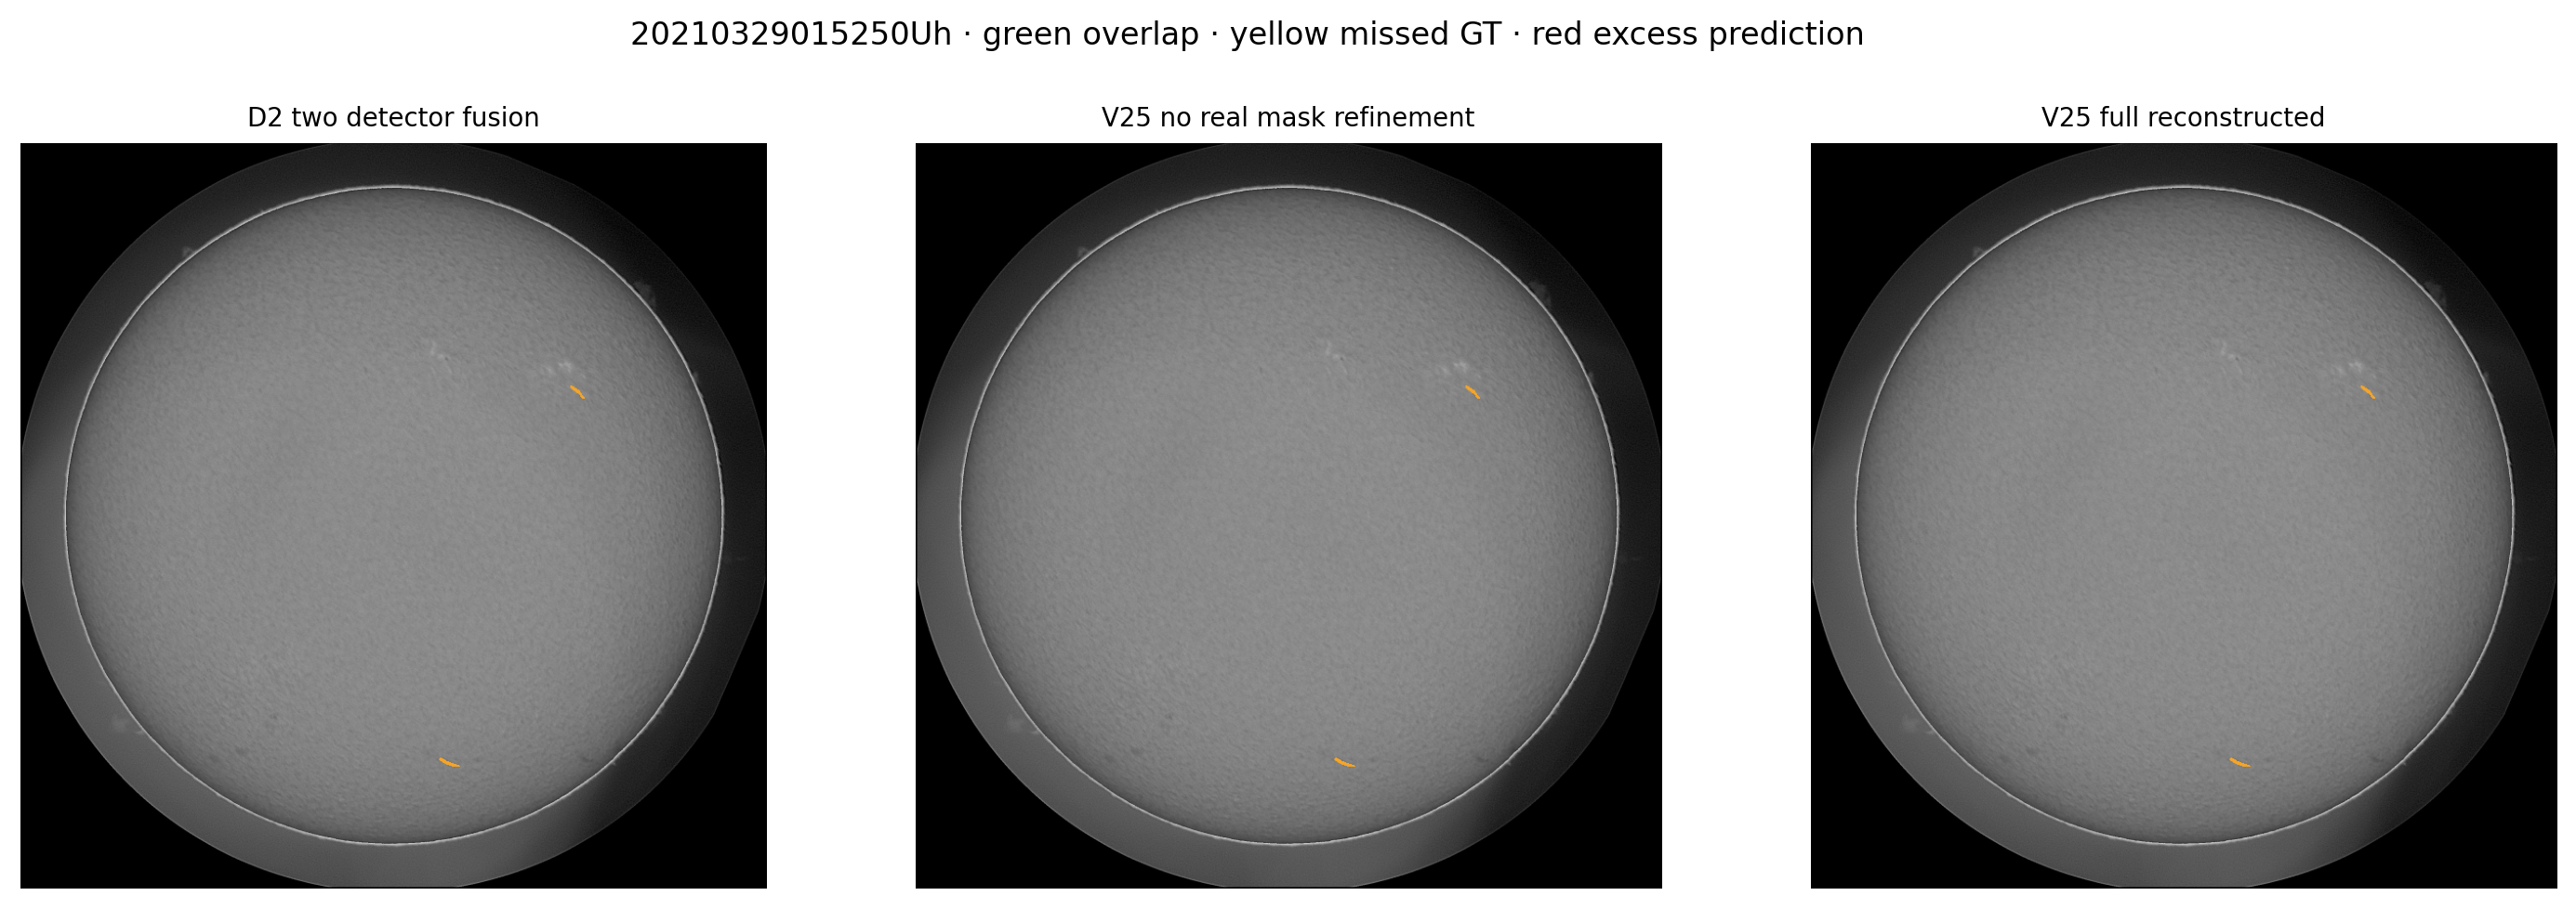
\includegraphics[width=\columnwidth]{case_error.png}
\caption{Actual labeled solar observation with detector-only, without-refinement, and reconstructed-full masks. Green denotes predicted/annotated overlap, amber missed foreground and red excess foreground.}\label{fig:cases}
\end{figure}

\subsection{Why candidate recovery did not generalize}
In V28, a solar-pretrained native-resolution expert model added an independent high-resolution proposal stream, but that model alone achieved only 0.3213 local PQ versus the frozen V25 reference of 0.4589. A conservative fusion changed the historical-audit PQ by just +0.0003, and a learned gate did not improve it. In V29, a four-estimator novelty-credit ranking system was trained to identify plausible novel instances not matched by V25. The candidate bank had 61 qualifying positives among 363 calibration examples, but the best policy gained just +0.0008 historical-audit PQ. Both failed preset evidence-based promotion gates and were not substituted for the exact 0.39-scored artifact. These later experiments show that candidate existence does not suffice: false positives, overlaps, and duplicate identity impose a quantifiable penalty.

\subsection{Reproducibility, computational constraints, and release}
The method uses two 22.36M-parameter solar YOLO11m models, a 13.75M-parameter V24 prompt refiner, a 0.99M-parameter curve specialist, a 69-feature rank ensemble, and a 13.75M-parameter real-mask refiner. Inputs are 2048-pixel H$\alpha$ images; results are compressed, nonoverlapping COCO RLE masks with unique instance IDs. Recorded hashes identify all seven model assets. The downloaded research-evidence bundle itself does not contain these trained weights; they must be provided publicly in the final repository. The final audit inference plus all component variants averaged 13.89 seconds per image with shared caching, \emph{not} standalone inference latency. A notebook reports source hashes, package versions, archival artifact identity, and matched-mask reproduction checks. The expanded technical history records V1--V29 hypotheses and their failed alternatives.

\begin{figure}[t]
\centering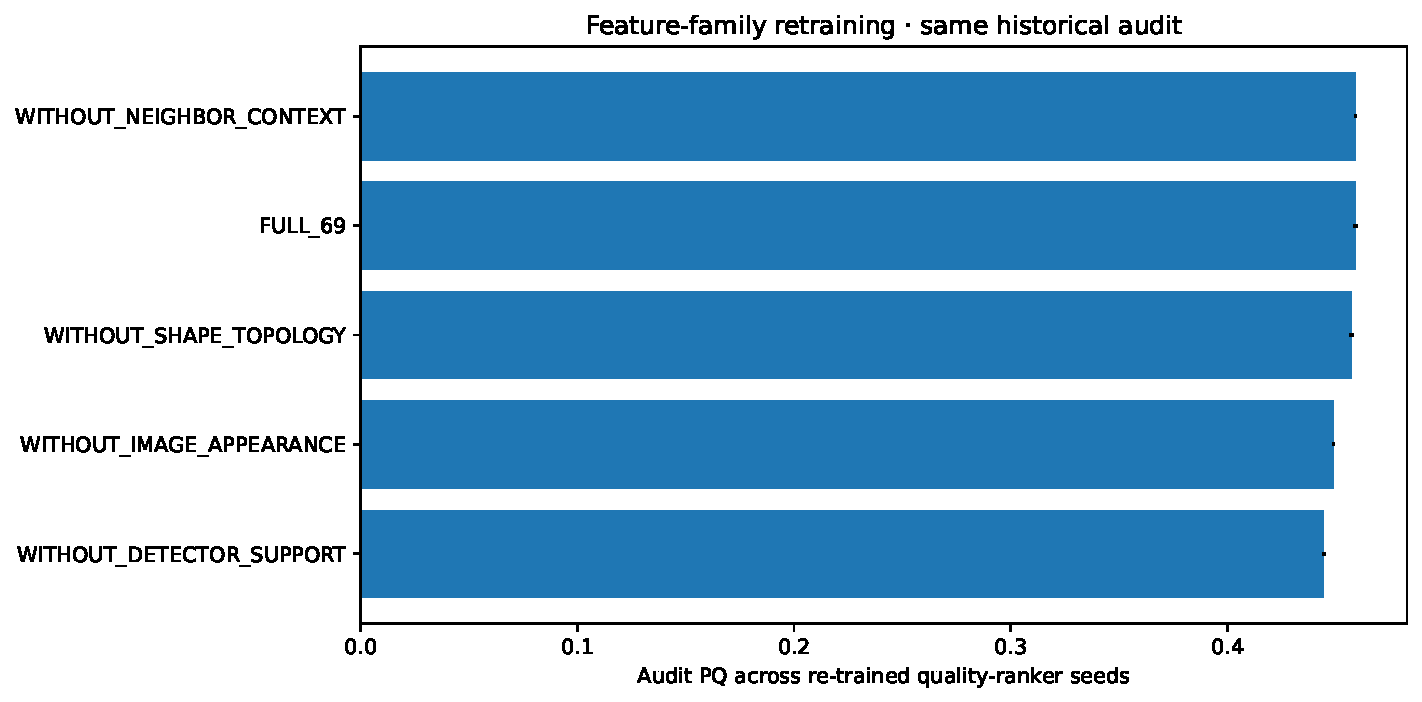
\includegraphics[width=.96\columnwidth]{feature_ablation.pdf}
\caption{Three-seed feature-family refit ablations: detector-support and local-appearance features are most influential for the quality ranker.}\label{fig:feature}
\end{figure}
\subsection{Limitations and reproducibility}
The strongest supported claim is that quality selection and selective refinement improve local PQ under fixed checkpoints. The optional addition of curve detections \emph{decreases} PQ in the reported audit. The 0.39 public score is a distinct user-reported Kaggle display value for the exact archived CSV. The historical audit was reused across iterations; no independent held-out dataset, repeat training of deep networks across seeds, or official-scoring parity test is claimed. Full source, package fingerprints, checkpoint identifiers, output schemas, and figure assets are provided for replication; to reproduce inference, the original trained checkpoints must accompany the repository.

\section{Acknowledgment}\label{sec:acknowledgment}
The organization of the Filament Segmentation Challenge 2026 is partially supported by the U.S. National Science Foundation (NSF) under Grant No. 2209912 and 2433781, directorate for Computer and Information Science and Engineering (CSE), and Office of Advanced Cyberinfrastructure (OAC), and Grant No. 2511630, AST Division Of Astronomical Sciences and MPS Directorate for Mathematical and Physical Sciences.

The Filament Segmentation Challenge 2026 is sponsored by the U.S. National Science Foundation (NSF) National Solar Observatory (NSO).

This work utilizes GONG data obtained by the NSO Integrated Synoptic Program, managed by the National Solar Observatory, which is operated by the Association of Universities for Research in Astronomy (AURA), Inc. under a cooperative agreement with the National Science Foundation and with contribution from the National Oceanic and Atmospheric Administration. The GONG network of instruments is hosted by the Big Bear Solar Observatory, High Altitude Observatory, Learmonth Solar Observatory, Udaipur Solar Observatory, Instituto de Astrof\'isica de Canarias, and Cerro Tololo Interamerican Observatory.

\bibliographystyle{ACM-Reference-Format}
\bibliography{main}
\end{document}
